% Parseval: retained coefficients and the orthogonal error.
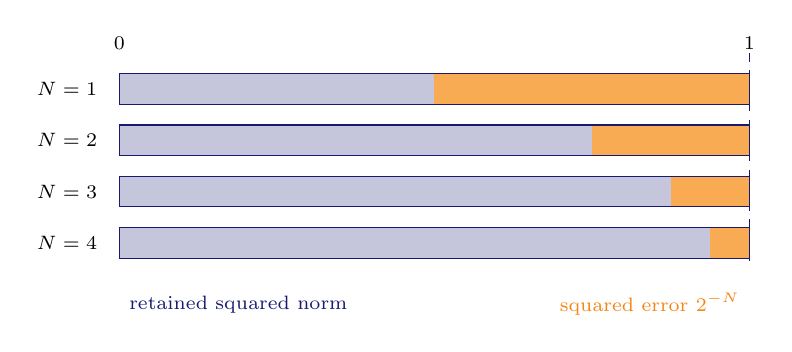
\begin{tikzpicture}[x=8cm,y=0.65cm,every node/.style={font=\scriptsize}]
\foreach \n in {1,...,4}{
\pgfmathsetmacro{\kept}{1-pow(2,-\n)}
\fill[MidnightBlue!25] (0,-\n) rectangle (\kept,-\n+0.6);
\fill[BurntOrange!65] (\kept,-\n) rectangle (1,-\n+0.6);
\draw[MidnightBlue] (0,-\n) rectangle (1,-\n+0.6);
\node[anchor=east] at (-0.02,-\n+0.3) {$N=\n$};
}
\node[MidnightBlue,anchor=west] at (0,-4.9) {retained squared norm};
\node[BurntOrange,anchor=east] at (1,-4.9) {squared error $2^{-N}$};
\node at (0,0.2) {$0$};\node at (1,0.2) {$1$};
\draw[MidnightBlue,dashed] (1,0)--(1,-4.1);
\end{tikzpicture}
